\documentclass[tikz,border=8pt]{standalone}

\usepackage[T1]{fontenc}
\usepackage{lmodern}
\usetikzlibrary{arrows.meta}

\begin{document}
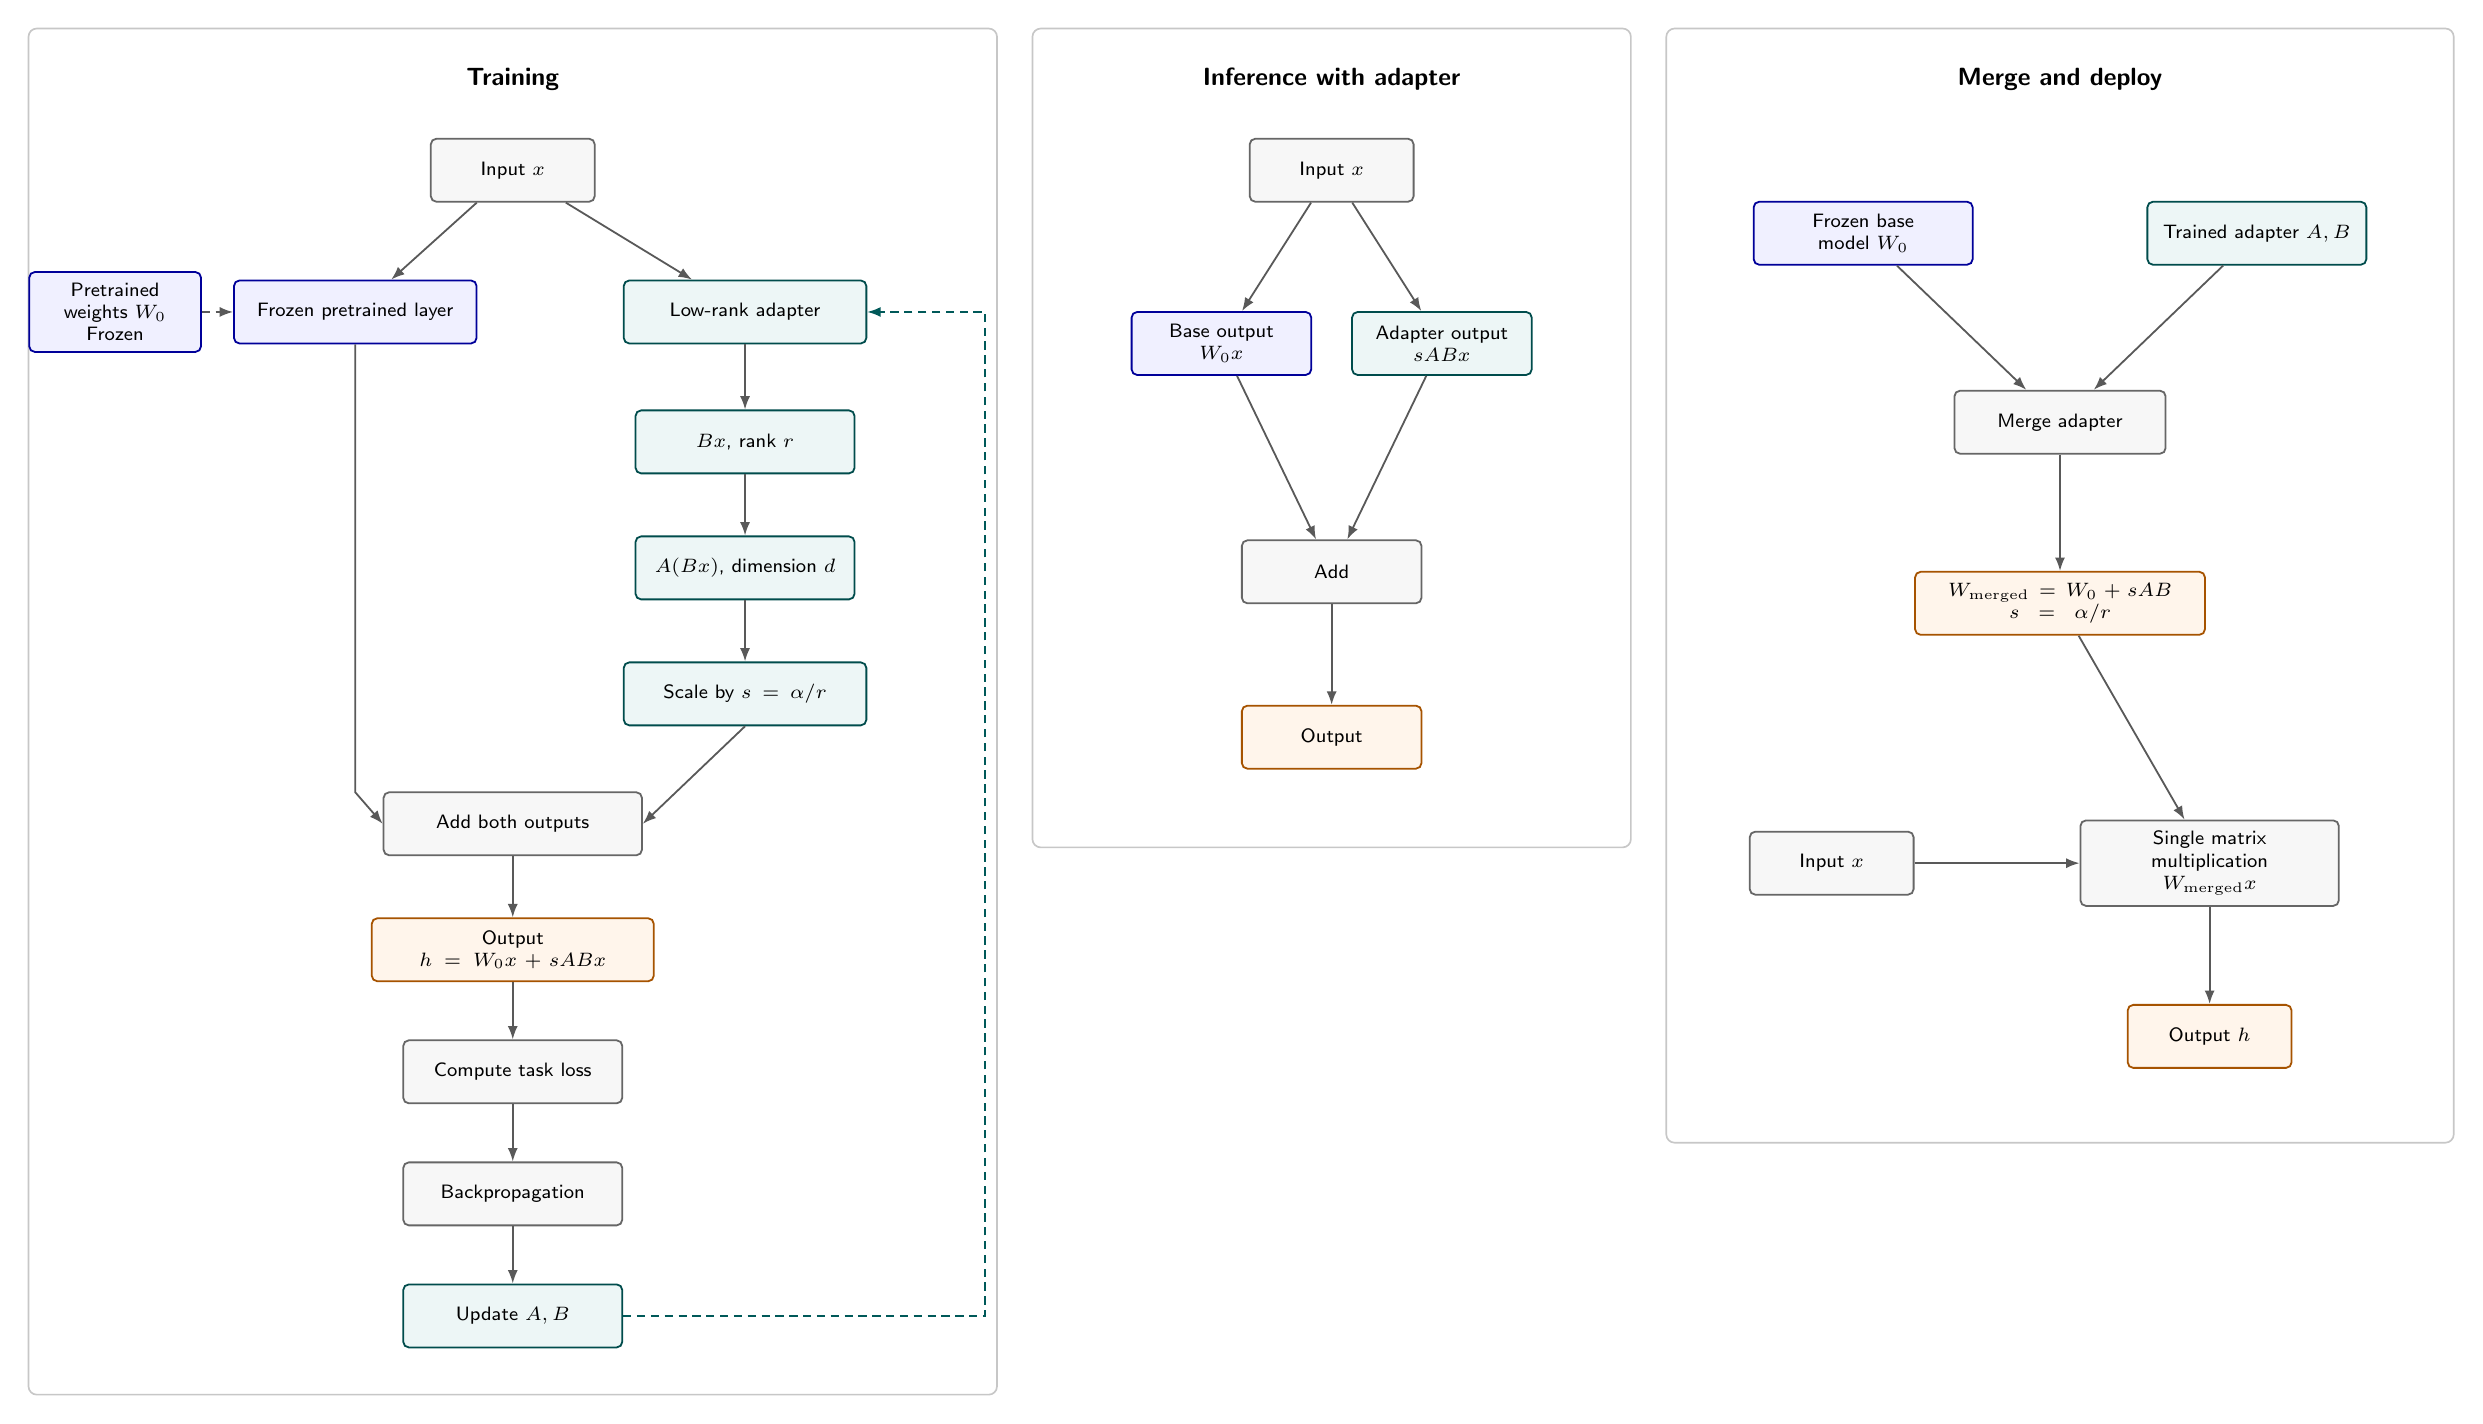
\begin{tikzpicture}[
  x=1cm,
  y=1cm,
  font=\sffamily\scriptsize,
  block/.style={
    draw=black!60,
    fill=black!3,
    rounded corners=2pt,
    line width=0.65pt,
    minimum height=8mm,
    text width=2.5cm,
    align=center,
    inner sep=4pt,
  },
  frozen/.style={block, draw=blue!60!black, fill=blue!6},
  adapter/.style={block, draw=teal!60!black, fill=teal!7},
  result/.style={block, draw=orange!65!black, fill=orange!8},
  panel/.style={draw=black!22, fill=white, rounded corners=3pt, line width=0.6pt},
  arrow/.style={draw=black!65, line width=0.65pt, -{Latex[length=1.7mm]}},
  frozen-link/.style={arrow, densely dashed},
  feedback/.style={arrow, densely dashed, draw=teal!70!black},
]

% Training panel: the frozen path and trainable low-rank path are summed.
\draw[panel] (0.0,0.0) rectangle (12.3,-17.35);
\node[font=\sffamily\bfseries\small] at (6.15,-0.65) {Training};

\node[block, text width=1.8cm] (train-input) at (6.15,-1.8) {Input \(x\)};
\node[frozen, text width=2.8cm] (base) at (4.15,-3.6) {Frozen pretrained layer};
\node[adapter, text width=2.8cm] (lowrank) at (9.1,-3.6) {Low-rank adapter};
\node[frozen, text width=1.9cm] (weights) at (1.1,-3.6)
  {Pretrained weights \(W_0\)\\Frozen};

\draw[arrow] (train-input) -- (base);
\draw[arrow] (train-input) -- (lowrank);
\draw[frozen-link] (weights.east) -- (base.west);

\node[adapter] (bproj) at (9.1,-5.25) {\(Bx\), rank \(r\)};
\node[adapter] (aproj) at (9.1,-6.85) {\(A(Bx)\), dimension \(d\)};
\node[adapter, text width=2.8cm] (scale) at (9.1,-8.45)
  {Scale by \(s=\alpha/r\)};
\node[block, text width=3.0cm] (sum) at (6.15,-10.1) {Add both outputs};
\draw[arrow] (lowrank) -- (bproj);
\draw[arrow] (bproj) -- (aproj);
\draw[arrow] (aproj) -- (scale);
\draw[arrow] (base.south) -- (4.15,-9.7) -- (sum.west);
\draw[arrow] (scale.south) -- (sum.east);

\node[result, text width=3.3cm] (train-output) at (6.15,-11.7)
  {Output\\\(h=W_0x+sABx\)};
\node[block] (loss) at (6.15,-13.25) {Compute task loss};
\node[block] (backprop) at (6.15,-14.8) {Backpropagation};
\node[adapter] (update) at (6.15,-16.35) {Update \(A,B\)};
\draw[arrow] (sum) -- (train-output);
\draw[arrow] (train-output) -- (loss);
\draw[arrow] (loss) -- (backprop);
\draw[arrow] (backprop) -- (update);
\draw[feedback] (update.east) -- ++(4.6,0) |- (lowrank.east);

% Unmerged inference panel.
\draw[panel] (12.75,0.0) rectangle (20.35,-10.4);
\node[font=\sffamily\bfseries\small] at (16.55,-0.65) {Inference with adapter};
\node[block, text width=1.8cm] (infer-input) at (16.55,-1.8) {Input \(x\)};
\node[frozen, text width=2.0cm] (base-out) at (15.15,-4.0) {Base output\\\(W_0x\)};
\node[adapter, text width=2.0cm] (adapter-out) at (17.95,-4.0) {Adapter output\\\(sABx\)};
\node[block, text width=2.0cm] (add) at (16.55,-6.9) {Add};
\node[result, text width=2.0cm] (infer-output) at (16.55,-9.0) {Output};
\draw[arrow] (infer-input) -- (base-out);
\draw[arrow] (infer-input) -- (adapter-out);
\draw[arrow] (base-out) -- (add);
\draw[arrow] (adapter-out) -- (add);
\draw[arrow] (add) -- (infer-output);

% Merge-and-deploy panel.
\draw[panel] (20.8,0.0) rectangle (30.8,-14.15);
\node[font=\sffamily\bfseries\small] at (25.8,-0.65) {Merge and deploy};
\node[frozen, text width=2.5cm] (trained-base) at (23.3,-2.6)
  {Frozen base model \(W_0\)};
\node[adapter, text width=2.5cm] (trained-adapter) at (28.3,-2.6)
  {Trained adapter \(A,B\)};
\node[block, text width=2.4cm] (merge) at (25.8,-5.0) {Merge adapter};
\node[result, text width=3.4cm] (merged) at (25.8,-7.3)
  {\(W_{\mathrm{merged}}=W_0+sAB\)\\\(s=\alpha/r\)};
\node[block, text width=1.8cm] (merged-input) at (22.9,-10.6) {Input \(x\)};
\node[block, text width=3.0cm] (multiply) at (27.7,-10.6)
  {Single matrix multiplication\\\(W_{\mathrm{merged}}x\)};
\node[result, text width=1.8cm] (merged-output) at (27.7,-12.8) {Output \(h\)};
\draw[arrow] (trained-base) -- (merge);
\draw[arrow] (trained-adapter) -- (merge);
\draw[arrow] (merge) -- (merged);
\draw[arrow] (merged) -- (multiply);
\draw[arrow] (merged-input) -- (multiply);
\draw[arrow] (multiply) -- (merged-output);
\end{tikzpicture}
\end{document}
